\section{Results \& evaluation}
\subsection{Correctness}
As stated earlier, the filesystem was split into two parts: a filesystem logic part (the \textit{adafs} package), and an I/O part (the \textit{disk} package).
Because the logic part is easier to verify, it was the primary focus of formal verification for this project.
Currently, approximately 25\% of the filesystem is verified, and most of the unverified code is in the \textit{disk} package.
Since the FUSE driver is written in C, and in Ada with C types, it is also not verified.

Subprograms were given functional and data contracts, and type definitions according to their expected functionality.
Although this does not formally verify the functionality of the entire filesystem, it is a good starting point.
\autoref{code:prover summary} shows a summary of the conducted checks, and \autoref{code:prover output} shows some of the locations of various checks.

\begin{lstlisting}[basicstyle=\tiny, caption={Prover summary (\textnormal{gnatprove})}, label={code:prover summary}]
Summary of SPARK analysis
=========================

----------------------------------------------------------------------------------------------------------
SPARK Analysis results   Total        Flow   CodePeer                       Provers   Justified   Unproved
----------------------------------------------------------------------------------------------------------
Data Dependencies            5           5          .                             .           .          .
Flow Dependencies            4           4          .                             .           .          .
Initialization               1           1          .                             .           .          .
Non-Aliasing                 .           .          .                             .           .          .
Run-time Checks             17           .          .    17 (CVC4 89%, Trivial 11%)           .          .
Assertions                   2           .          .                      2 (CVC4)           .          .
Functional Contracts         6           .          .      6 (CVC4 92%, Trivial 8%)           .          .
LSP Verification             .           .          .                             .           .          .
Termination                  .           .          .                             .           .          .
Concurrency                  .           .          .                             .           .          .
----------------------------------------------------------------------------------------------------------
Total                       35    10 (29%)          .                      25 (71%)           .          .

max steps used for successful proof: 1

Analyzed 12 units
\end{lstlisting}

\begin{lstlisting}[basicstyle=\tiny, caption={Excerpt from the prover output (\textnormal{gnatprove})}, label={code:prover output}]
adafs-inode.adb:6:27: info: division check proved (CVC4: 1 VC in max 0.0 seconds and 1 step)
adafs-inode.adb:6:27: info: range check proved (CVC4: 1 VC in max 0.0 seconds and 1 step)
adafs-inode.adb:8:44: info: division check proved (CVC4: 1 VC in max 0.0 seconds and 1 step)
adafs-inode.adb:13:12: info: overflow check proved (CVC4: 1 VC in max 0.0 seconds and 1 step)
adafs-inode.adb:14:12: info: division check proved (CVC4: 1 VC in max 0.0 seconds and 1 step)
adafs-inode.adb:14:12: info: range check proved (CVC4: 1 VC in max 0.0 seconds and 1 step)
adafs-inode.adb:14:28: info: overflow check proved (CVC4: 1 VC in max 0.0 seconds and 1 step)
adafs-inode.ads:40:60: info: range check proved (CVC4: 1 VC in max 0.0 seconds and 1 step)
adafs-inode.ads:66:10: info: data dependencies proved
adafs-inode.ads:67:10: info: flow dependencies proved
adafs-inode.ads:69:18: info: postcondition proved (CVC4: 2 VC in max 0.0 seconds and 1 step)
adafs-proc.adb:6:14: info: discriminant check proved (CVC4: 2 VC in max 0.0 seconds and 1 step)
adafs-proc.adb:12:16: info: discriminant check proved (CVC4: 2 VC in max 0.0 seconds and 1 step)
adafs-proc.ads:26:05: info: data dependencies proved
adafs-filp.adb:18:30: info: loop invariant initialization proved (CVC4: 1 VC in max 0.0 seconds and 1 step)
adafs-filp.adb:18:30: info: loop invariant preservation proved (CVC4: 1 VC in max 0.0 seconds and 1 step)
adafs-filp.ads:28:13: info: postcondition proved (CVC4: 3 VC in max 0.0 seconds and 1 step)
adafs-filp.ads:32:28: info: initialization of "free_fd" proved
adafs-filp.ads:33:05: info: data dependencies proved
adafs-filp.ads:34:05: info: flow dependencies proved
adafs-filp.ads:35:13: info: postcondition proved (CVC4: 2 VC in max 0.0 seconds and 1 step)
\end{lstlisting}

The checks done by the prover can each be related directly to a Common Weakness Enumeration (CWE) number; these are shown in \autoref{tab:checks and cwe numbers} \cite{sparkUG}.

\begin{table}[h]
  \centering
  \vspace{1em}
  \renewcommand{\arraystretch}{1.5}
  \begin{tabular}{| l | l |}
    \hline
    \textbf{Message} & \textbf{CWE number} \\ \hline
    divide by zero & 369 \\ \hline
    index check & 120 \\ \hline
    overflow check & 190 \\ \hline
    fp\_overflow check & 739 \\ \hline
    range check & 682 \\ \hline
    predicate check & 682 \\ \hline
    predicate check on default value & 682 \\ \hline
    null pointer dereference & 476 \\ \hline
    memory leak & 401 \\ \hline
    memory leak at end of scope & 401 \\ \hline
    discriminant check & 136 \\ \hline
    tag check & 136 \\ \hline
    use of an uninitialized variable & 457 \\ \hline
    precondition & 628 \\ \hline
    postcondition & 682 \\ \hline
  \end{tabular}
  \renewcommand{\arraystretch}{1}
  \vspace{1em}
  \caption{SPARK checks with their respective CWE numbers}
  \label{tab:checks and cwe numbers}
\end{table}

Due to Ada's type system, many of the checks do not take much effort to verify; in fact, all of the conducted checks were verified in one step.
The assurances provided by the prover are powerful, as they mean that e.g. overflow errors and range errors can \textit{never} happen at those locations.
In standard Ada, instructions are emitted to check that e.g. array accesses are within the bounds of the array.
However, with SPARK, such verifications can be conducted ahead of time.
This means that the runtime checks done by Ada can be safely disabled, eliminating a number of machine instructions and thus improving the performance of the system.

\subsection{Performance}
We compare the performance of AdaFS with a C implementation of a FUSE-based MINIX 3 filesystem, fuse-mfs\footnote{\url{https://github.com/redcap97/fuse-mfs}}.
As AdaFS is not a complete filesystem, but only supports a small set of operations, it was not possible to use a standardised utility to test it.
Therefore, we created a microbenchmark in C that executes the relevant system calls and counts the number of CPU clock cycles necessary for each operation.
We compared some common filesystem operations, such as creating, writing, reading, and deleting files.
We used a virtual machine in VirtualBox 6.1.10 on a macOS host, running Debian 4.19.118, with FUSE version 3.4.1.
The machine has 4 CPUs, 2 GB of RAM, and a Intel Core i7-3615QM processor at 2.3 GHz.
The disk images for the filesystem were stored on an SSD.

To calculate the number of CPU clock cycles an operation takes, we use a deterministic version of the ReaD Time Stamp Counter (RDTSC) instruction, RDTSCP, which is added as inline assembly in the C microbenchmark code.
The code to calculate elapsed clock cycles is shown in \autoref{code:rdtsc}.

\begin{lstlisting}[caption={Calculating clock cycles}, label={code:rdtsc}, language=C]
static __inline__ int64_t rdtsc_s(void) {
  unsigned a, d;
  asm volatile("cpuid" ::: "%rax", "%rbx", "%rcx", "%rdx");
  asm volatile("rdtsc" : "=a" (a), "=d" (d));
  return ((unsigned long)a) | (((unsigned long)d) << 32);
}

static __inline__ int64_t rdtsc_e(void) {
  unsigned a, d;
  asm volatile("rdtscp" : "=a" (a), "=d" (d));
  asm volatile("cpuid" ::: "%rax", "%rbx", "%rcx", "%rdx");
  return ((unsigned long)a) | (((unsigned long)d) << 32);
}
typedef int64_t cycle_t;

int main() {
  cycle_t cycles_before, cycles_after, cycles_per;
  cycles_before = rdtsc_s();
  // Call the test function here...
  cycles_after = rdtsc_e();
  cycles_per = cycles_after-cycles_before;
  printf("CPU cycles: %ld\n", cycles_per);
}
\end{lstlisting}

We choose RDTSCP instead of RDTSC because the CPU cannot reorder it relative to other instructions, as this reordering would cause noise in our results \cite{delorie2016}.
We set the \lstinline{isolcpus} kernel option at boot to isolate CPU 1, and then use the \lstinline{sched_affinity} function call to explicitly schedule each test on this CPU.
\autoref{code:schedule test} shows the code for this.

\begin{lstlisting}[caption={Schedule a test on CPU 1}, label={code:schedule test}, language=C]
#define _GNU_SOURCE
#include <sched.h>
void run_test(void) {
  // Schedule
  cpu_set_t the_cpu;
  int the_cpu_num = 1;
  CPU_ZERO(&the_cpu);
  CPU_SET(the_cpu_num, &the_cpu);
  if (sched_setaffinity(0, sizeof(the_cpu), &the_cpu) == -1) {
    perror("setaffinity failed");
  }

  // Run any tests below
  ...
}
\end{lstlisting}

We also assign interrupts to CPU 0 to avoid interference.
This ensures that no other processes are scheduled on the same CPU as our tests, i.e. that our results are as noiseless as possible.
We run FUSE in single-thread mode for both implementations of the filesystem.

We run the benchmark 30 times for each filesystem implementation; \autoref{tab:fs comparison} presents the median values for each implementation and operation.
It is apparent that AdaFS is significantly slower than fuse-mfs.
The largest difference is apparent in the create operation, which is approximately 412.5 times slower.
The remove operation is around 2.5 times slower than that of fuse-mfs.
For other operations, the difference is not as drastic, though the Ada implementation is still around 10-20\% slower on average.

\begin{table}[h]
  \begin{subtable}[t]{\textwidth}
    \centering
    \begin{tabular}{l r | r | r | r}
                      & \multicolumn{2}{c}{\underline{Create}}                                           & \multicolumn{2}{c}{\underline{Remove}} \\
       Implementation & Cycles                                 & Std. dev.                               & Cycles                   & Std. dev.                   \\
      \hline \hline
      AdaFS           & \result{adafs-create}                  & \result{adafs-create-stdev}             & \result{adafs-remove}    & \result{adafs-remove-stdev} \\
      fuse-mfs        & \result{fuse-mfs-create}               & \result{fuse-mfs-create-stdev}          & \result{fuse-mfs-remove} & \result{fuse-mfs-remove-stdev}
    \end{tabular}
    \caption{CPU cycles to create and remove files}
    \label{tab:create remove files}
  \end{subtable}

  \bigskip

  \begin{subtable}[t]{\textwidth}
    \centering
    \small
    \begin{tabular}{l r | r | r | r | r | r | r | r}
                     & \multicolumn{2}{c}{\underline{Read 1 B}} & \multicolumn{2}{c}{\underline{Read 1 KB}} & \multicolumn{2}{c}{\underline{Read 10 KB}} & \multicolumn{2}{c}{\underline{Read 100 KB}} \\
      Implementation & Cycles                                  & Std. dev.                                & Cycles                                    & Std. dev.                                   & Cycles                       & Std. dev.                          & Cycles                        & Std. dev.                        \\
      \hline \hline
      AdaFS          & \result{adafs-read-1}                   & \result{adafs-read-1-stdev}              & \result{adafs-read-1024}                  & \result{adafs-read-1024-stdev}              & \result{adafs-read-10240}    & \result{adafs-read-10240-stdev}    & \result{adafs-read-102400}    & \result{adafs-read-102400-stdev} \\
      fuse-mfs       & \result{fuse-mfs-read-1}                & \result{fuse-mfs-read-1-stdev}           & \result{fuse-mfs-read-1024}               & \result{fuse-mfs-read-1024-stdev}           & \result{fuse-mfs-read-10240} & \result{fuse-mfs-read-10240-stdev} & \result{fuse-mfs-read-102400} & \result{fuse-mfs-read-102400-stdev}
    \end{tabular}
    \caption{CPU cycles to read files of varying sizes}
    \label{tab:read files}
  \end{subtable}

  \bigskip

  \begin{subtable}[t]{\textwidth}
    \centering
    \small
    \begin{tabular}{l r | r | r | r | r | r | r | r}
                     & \multicolumn{2}{c}{\underline{Write 1 B}} & \multicolumn{2}{c}{\underline{Write 1 KB}} & \multicolumn{2}{c}{\underline{Write 10 KB}} & \multicolumn{2}{c}{\underline{Write 100 KB}} \\
      Implementation & Cycles                                  & Std. dev.                                & Cycles                                    & Std. dev.                                   & Cycles                       & Std. dev.                          & Cycles                        & Std. dev.                        \\
      \hline \hline
      AdaFS          & \result{adafs-write-1}                   & \result{adafs-write-1-stdev}              & \result{adafs-write-1024}                  & \result{adafs-write-1024-stdev}              & \result{adafs-write-10240}    & \result{adafs-write-10240-stdev}    & \result{adafs-write-102400}    & \result{adafs-write-102400-stdev} \\
      fuse-mfs       & \result{fuse-mfs-write-1}                & \result{fuse-mfs-write-1-stdev}           & \result{fuse-mfs-write-1024}               & \result{fuse-mfs-write-1024-stdev}           & \result{fuse-mfs-write-10240} & \result{fuse-mfs-write-10240-stdev} & \result{fuse-mfs-write-102400} & \result{fuse-mfs-write-102400-stdev}
    \end{tabular}
    \caption{CPU cycles to write files of varying sizes}
    \label{tab:write files}
  \end{subtable}
  \caption{Comparing filesystem operation performance in C (fuse-mfs) and Ada (AdaFS), showing the median and standard deviation across 30 observations.}
  \label{tab:fs comparison}
\end{table}

\autoref{fig:read comparison} and \autoref{fig:write comparison} show how the read and write operations scale with buffer size, respectively.
Excluding the fact that AdaFS is much slower overall, the implementations scale in a relatively similar manner.
The scaling of the read operation, shown in \autoref{fig:read comparison}, is essentially identical.
From \autoref{fig:write comparison}, we can discern some differences in the scaling of writes.
For example, writing a 10 KB file is faster than writing a 1 KB file in AdaFS, but the opposite is true for fuse-mfs.
Moreover, the number of cycles increases more rapidly with the file size in AdaFS tha it does in fuse-mfs.

\begin{figure}[h]
  \centering
  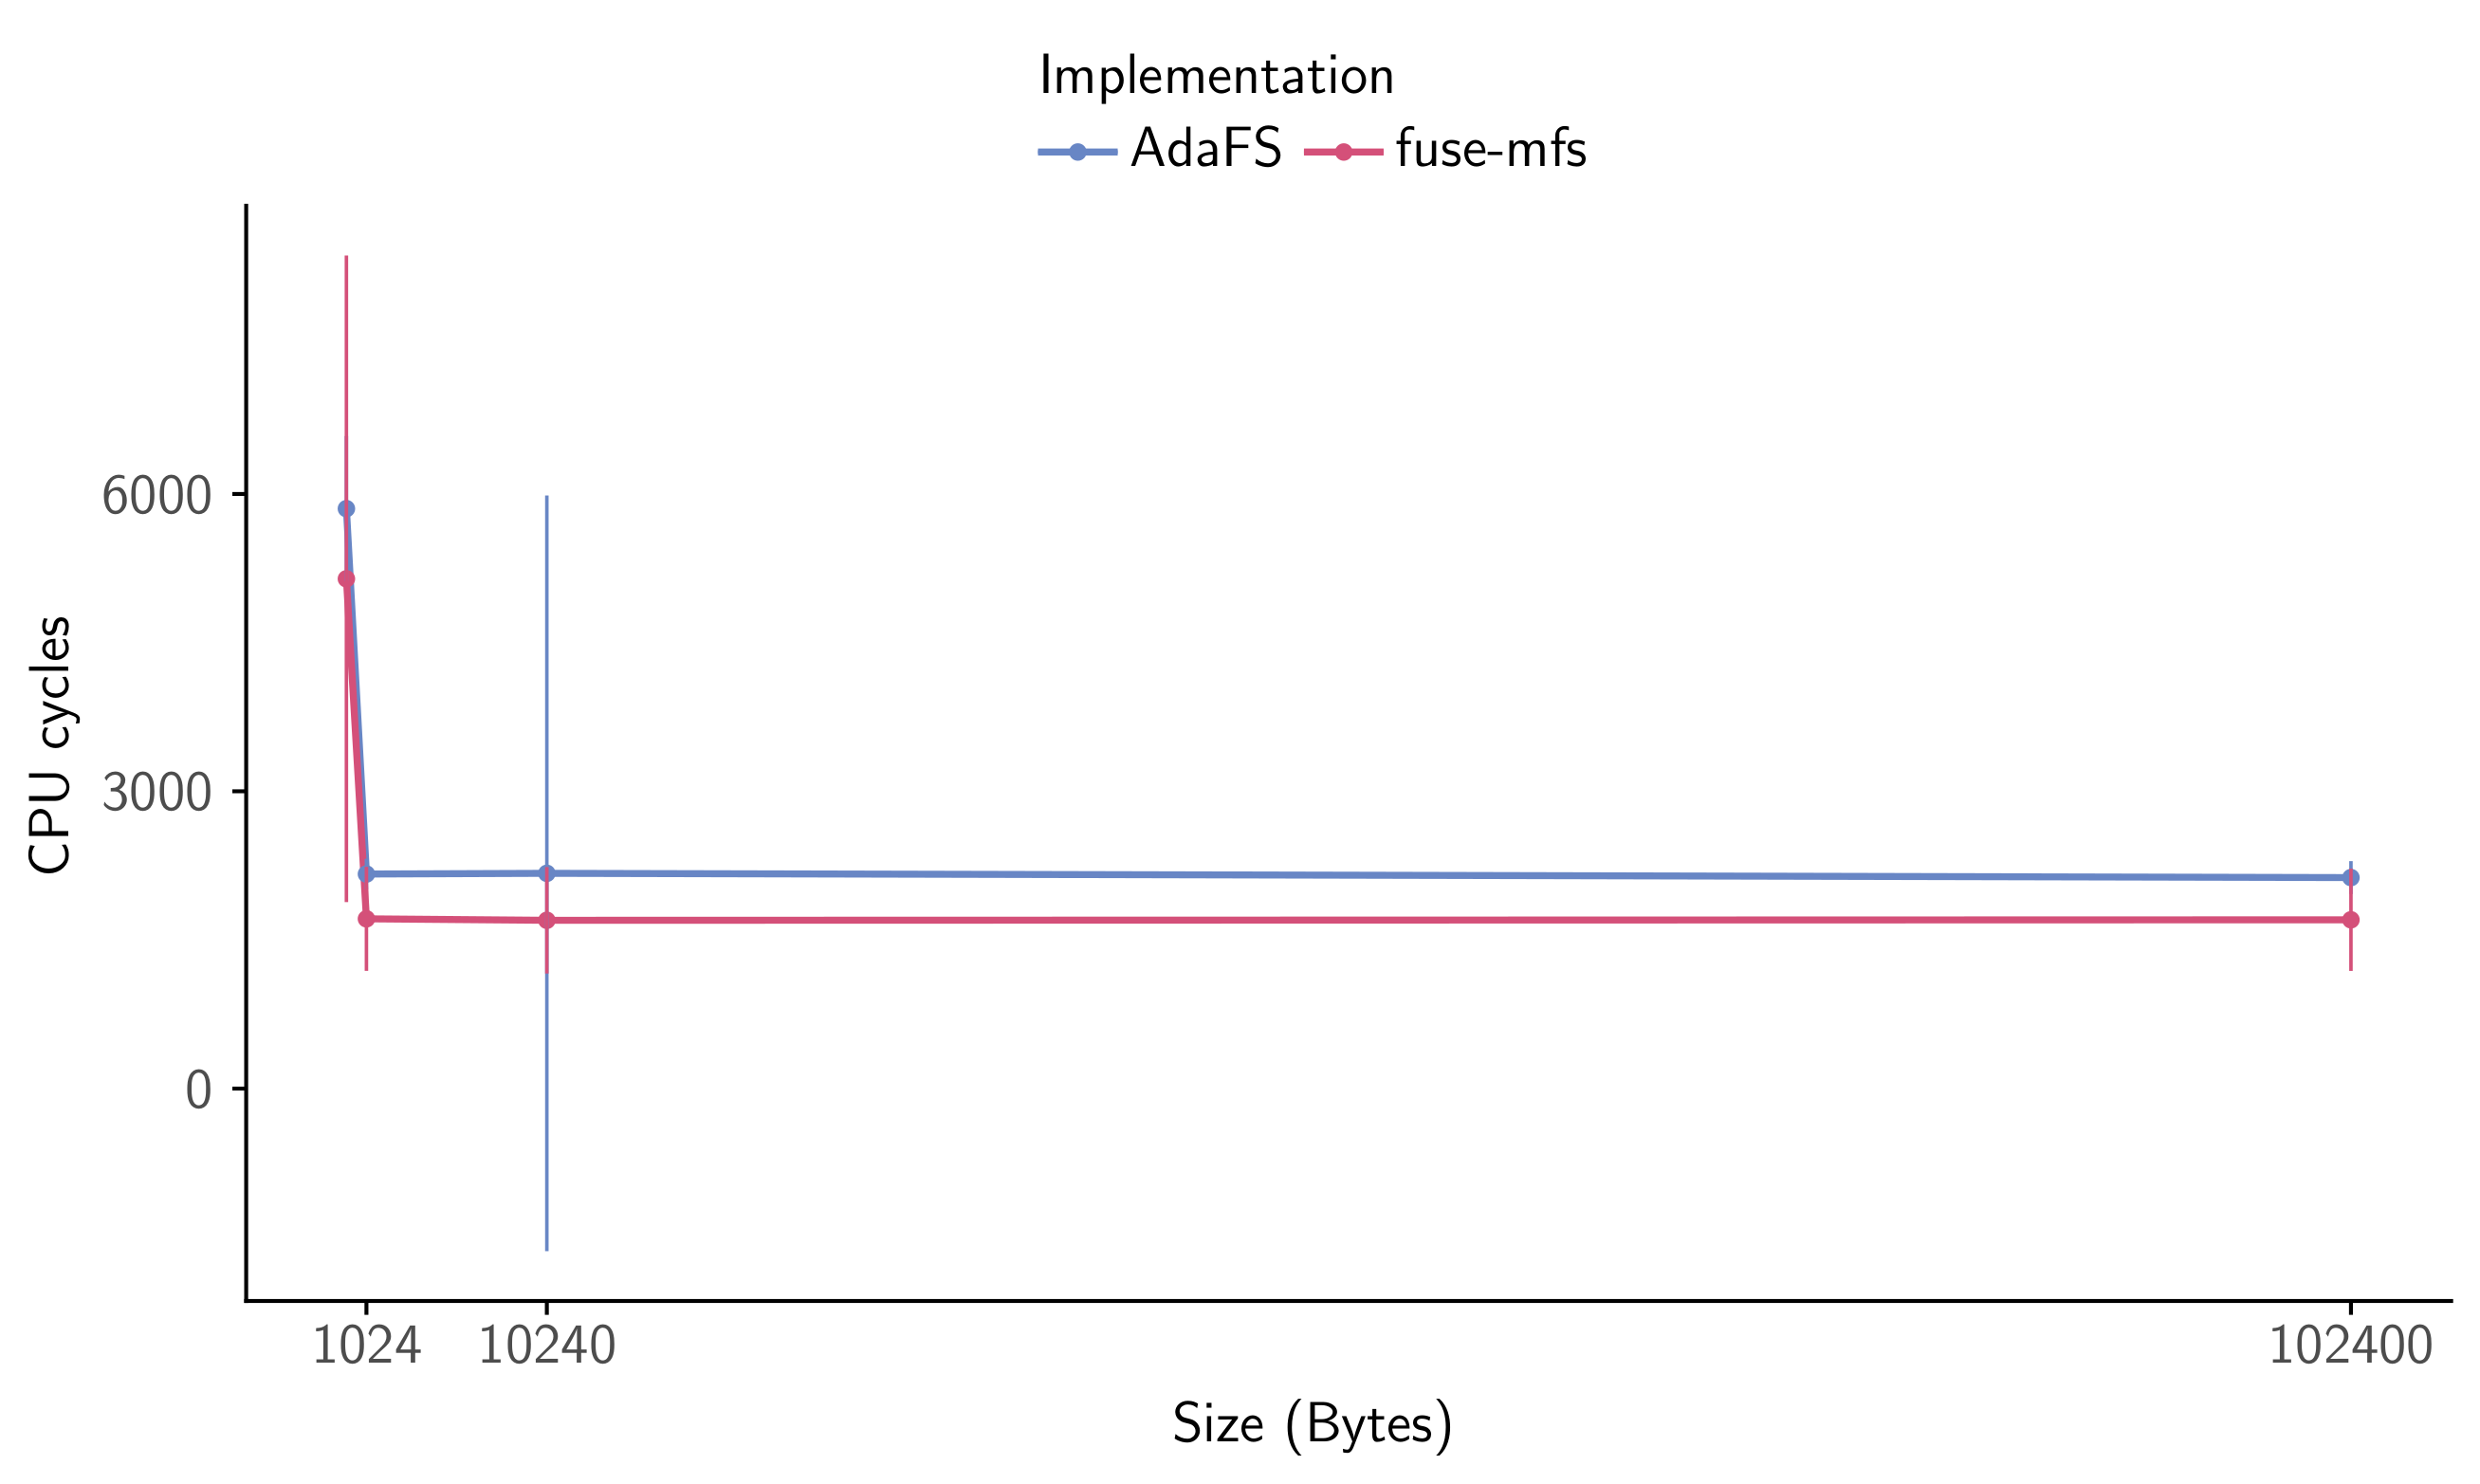
\includegraphics[scale=0.7]{read.png}
  \caption{Comparing file read performance in C (fuse-mfs) and Ada (AdaFS)}
  \label{fig:read comparison}
\end{figure}

\begin{figure}[h]
  \centering
  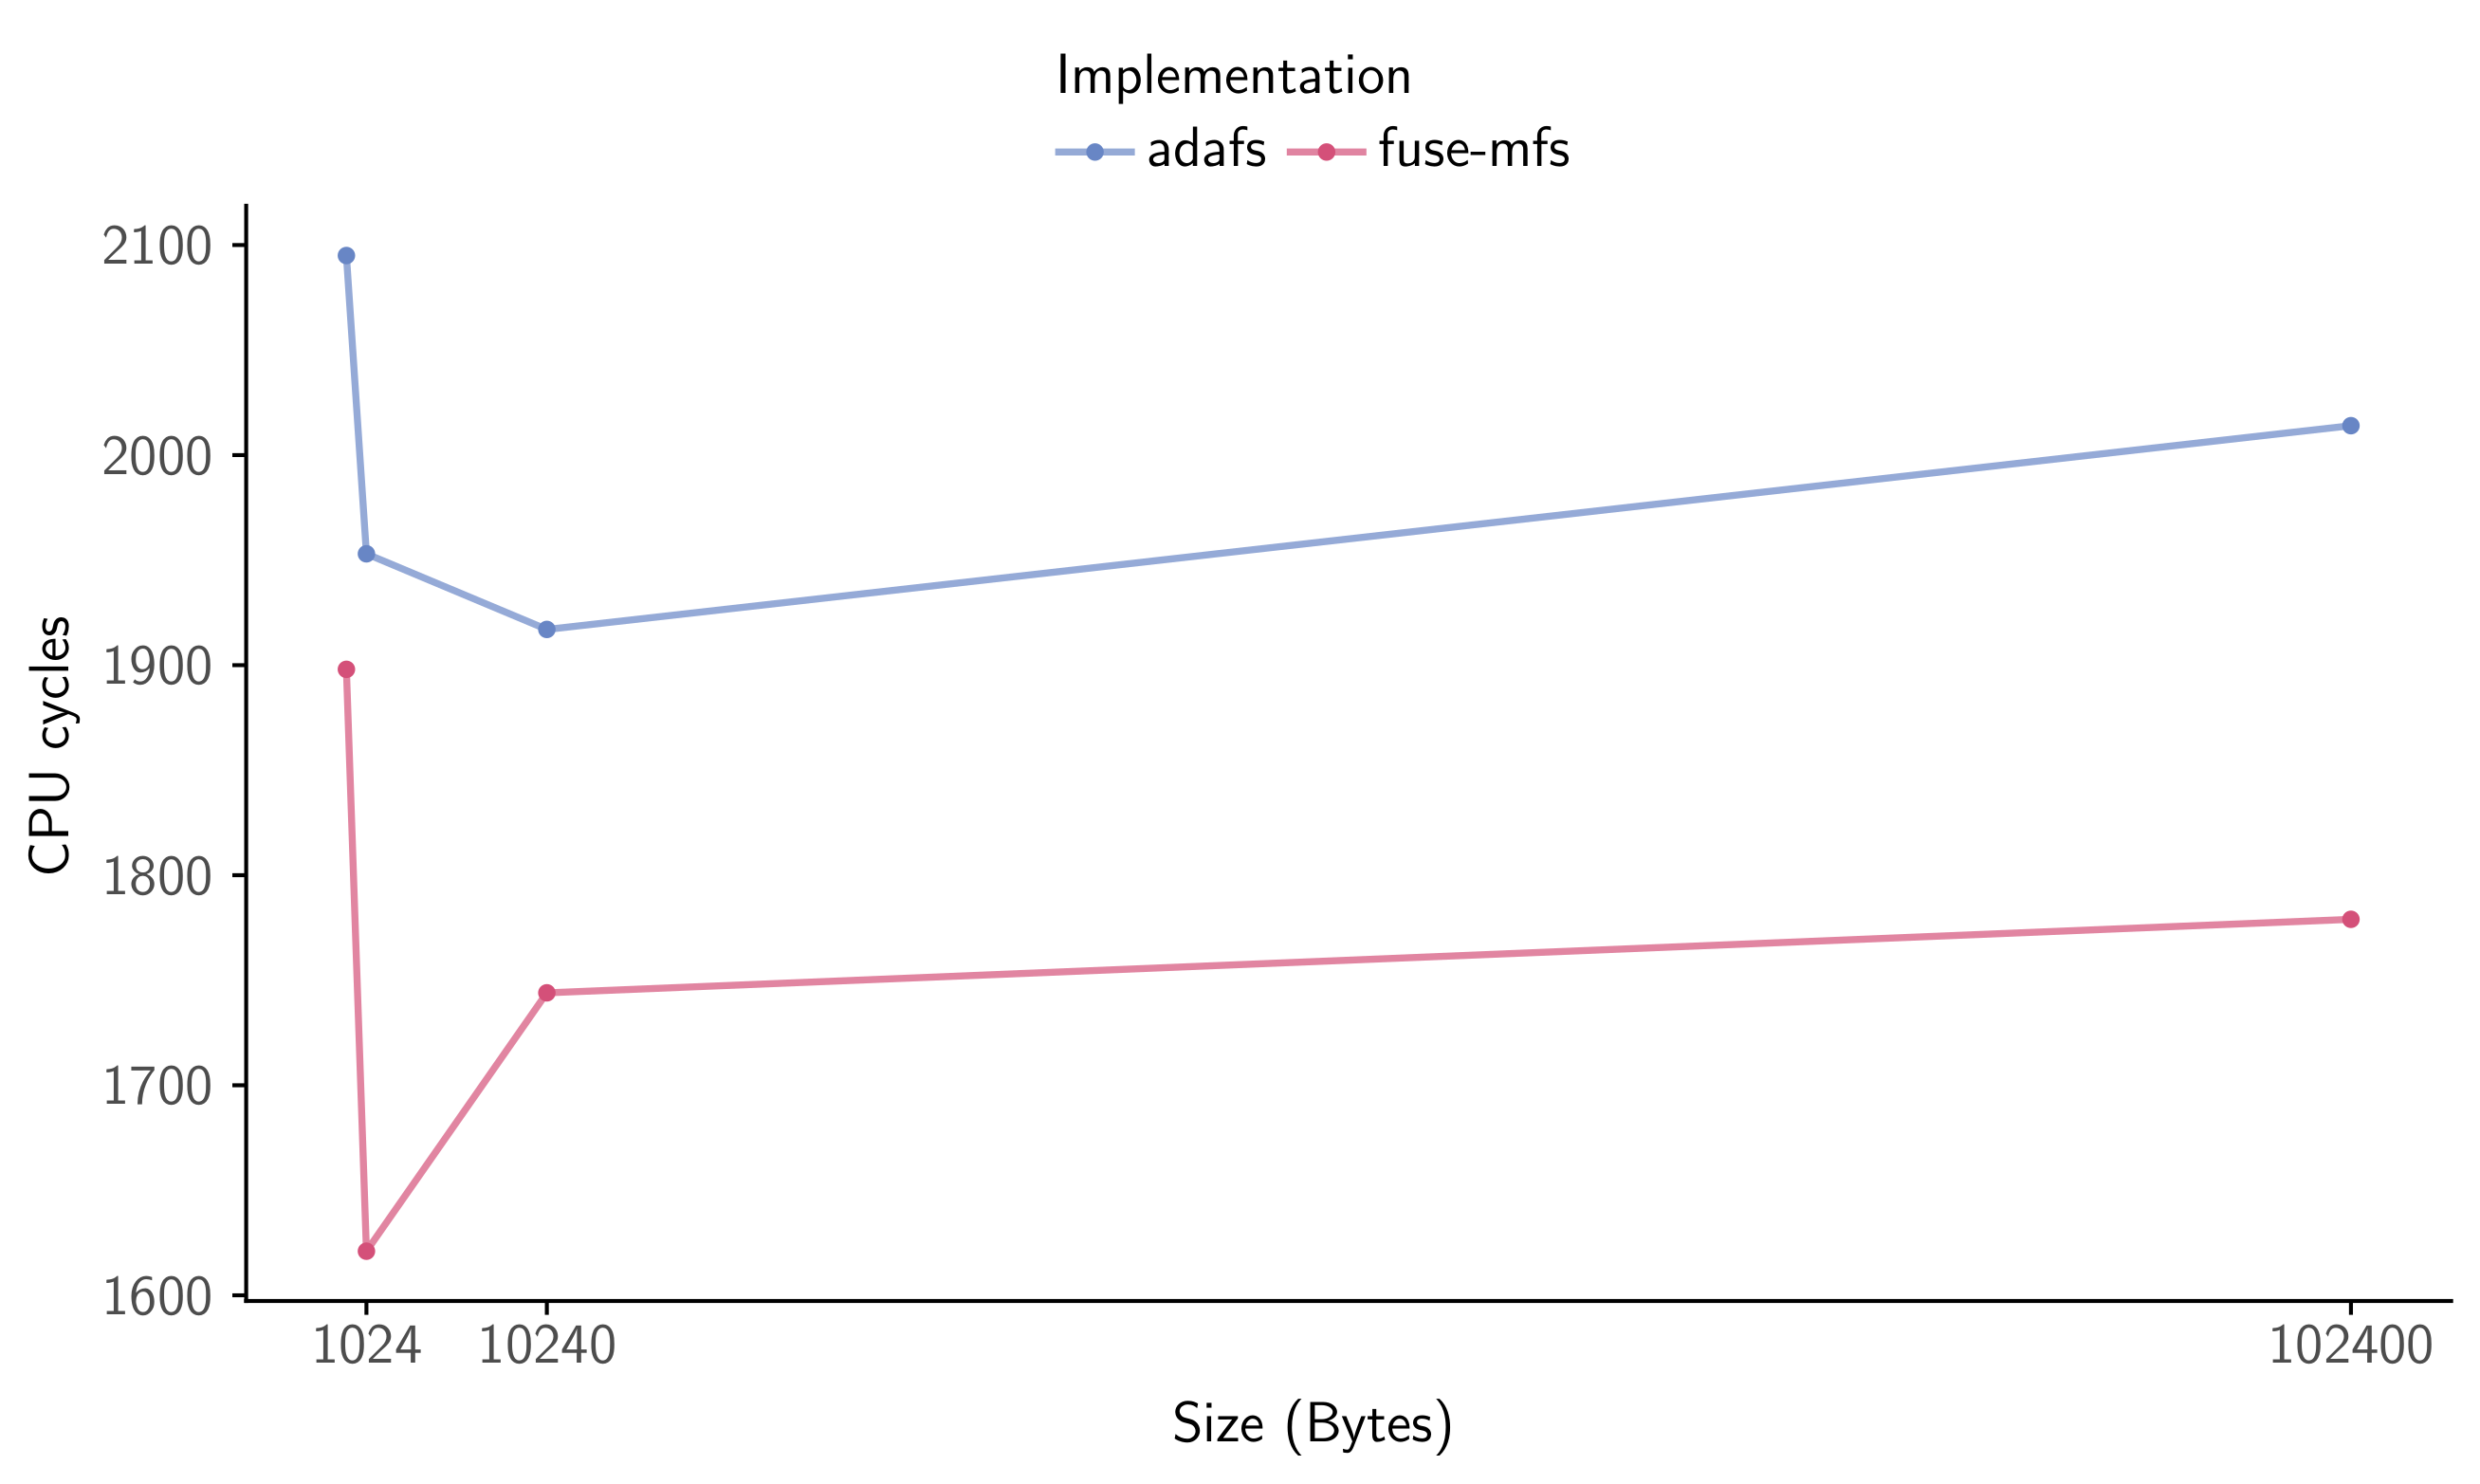
\includegraphics[scale=0.7]{write.png}
  \caption{Comparing file write performance in C (fuse-mfs) and Ada (AdaFS)}
  \label{fig:write comparison}
\end{figure}

These differences in performance are mostly small enough that they are not generally noticeable in everyday life.
However, a create operation that takes 0.24 seconds (548615020 cycles at 2.3 GHz) may have a visible impact, and the other operations may also cause issues in applications where speed is critical.
Thus, it is important to find out why this slowdown happens, or eliminate factors that do not cause decreased performance.
It may not necessarily be due to the extra code needed for formal verification; AdaFS does not employ any optimisations or caching that MINIX 2 uses, and MINIX 3 is even more optimised for speed than MINIX 2.

To determine if the verification code or implementation language may play a role in the slowdown, we implemented two versions of a factorial function for numbers up to 5, in C and Ada.
In Ada, we use the same settings and pragmas as AdaFS.
The Ada version of the function includes a full formal specification, with data and functional contracts, and with type definitions.
The Ada function is exported and called from C.
The C version follows the Ada version as closely as the language allows.

We run both implementations 500 times, counting the clock cycles.
The results (median and standard deviation) are shown in \autoref{tab:factorial comparison}.
From this, we can see that the Ada implementation only takes 8 more clock cycles than the C implementation.
Therefore, the implementation language and formal verification code are likely not major contributors to the decreased performance we see in AdaFS.
The performance degradation must thus be caused by other differences in the implementations.

\begin{table}[h]
  \centering
  \begin{tabular}{l | r | r}
    Implementation & Cycles & Std. dev. \\
    \hline \hline
    Ada            & 132    & 55.21     \\
    C              & 124    & 38.33
  \end{tabular}
  \caption{Factorial function comparison in Ada and C.}
  \label{tab:factorial comparison}
\end{table}
\clearpage
